%% ++++++++++++++++++++++++++++++++++++++++++++++++++++++++++++
%% Kapitel 2: Benötigte Software, Aufrufe
%% ++++++++++++++++++++++++++++++++++++++++++++++++++++++++++++
%
%  Gerüst:
%  * Version 0.11
%  * Dipl.-Ing. Karsten Renhak, karsten.renhak@tu-ilmenau.de
%  * Fachgebiet Kommunikationsnetze, TU Ilmenau
%
%  Für Hauptseminare, Studienarbeiten, Diplomarbeiten
%
%  Autor           : Max Mustermann
%  Letzte Änderung : 31.12.2011
%

\chapter{Software}
Dieses Kapitel zeigt, welche Programme zur Nutzung von \LaTeX\ 
benötigt werden. \LaTeX\ ist für alle Plattformen verfügbar,
allerdings unterscheiden sich die Paketnamen teilweise.



\section{Installation des Basissystems}
Eine vollständige \LaTeX"=Installation besteht aus mehreren Komponenten.
Zusätzlich zur absolut notwendigen Basisinstallation empfiehlt sich
noch die Installation diverser Hilfsprogramme, wie z.B. den
PDF"=Betrachter \emph{Acrobat Reader}, welcher weder Bestandteil des
\LaTeX"=Paketes ist noch zum Installationsumfang eines Windowssystems
gehört.



\subsection{Windows}
Bei Verwendung von Microsoft Windows werden mehrere Programmkomponenten benötigt,
siehe Tabelle \ref{tabelle:winsoftware}.

\begin{table}[ht!]
\centering
\begin{tabular}{lk{.45\textwidth}c}
\hline
Programmname &
Aufgabe &
Quelle
\tabularnewline
\hline
MiKTeX &
\LaTeX\ Distribution, DVI-Betrachter, incl. TeXworks Editor &
\cite{link:miktex}
\tabularnewline
TeX Live &
\LaTeX\ Distribution, DVI-Betrachter, incl. TeXworks Editor &
\cite{link:texlive}
\tabularnewline
Ghostview, Ghostscript &
Betrachter für PS-Dateien &
\cite{link:ghostview}
\tabularnewline
Acrobat Reader &
Betrachter für PDF-Dateien &
\cite{link:acrobatreader}
\tabularnewline
TeXnicCenter &
Entwicklungsumgebung &
\cite{link:texniccenter}
\tabularnewline
TeXworks &
Entwicklungsumgebung &
\cite{link:texworks}
\tabularnewline
\hline
\end{tabular}
\caption{Benötigte Programme unter Windows}
\label{tabelle:winsoftware}
\end{table}

\nomenclature{DVI}{\markup{D}e\markup{v}ice
                   \markup{I}ndependent, Dateiendung}
MiKTeX ist die \LaTeX"=Distribution für Microsoft Windows.
Sie enthält u.a. das Kommando {\ttfamily latex}, mit dessen Hilfe die {\ttfamily .tex} Dateien
in {\ttfamily .dvi} Dateien übersetzt werden können. Diese
\emph{Device Independent} (DVI) Dateien können bereits mit Hilfe
des DVI-Viewers angezeigt werden. Sinnvoll ist
allerdings eine anschließende Wandlung in Postscript
(\(\to \) {\ttfamily dvips}) oder in ein PDF.
"`BibTeX"' zur Handhabung von Literaturverzeichnissen,
{\ttfamily makeindex} zur Erzeugung von Abkürzungsverzeichnissen sowie
{\ttfamily pdflatex} zur direkten Erzeugung von PDF's aus \TeX"=Quellcodes sind ebenfalls bereits in MiKTeX enthalten.

Um Postscript"=Dateien unter Windows anzeigen zu können, werden die
Programme "`Ghostview"' und "`Ghostscript"' benötigt. Beide sind
unter \cite{link:ghostview} frei erhältlich.

Zur Anzeige von PDF's, egal ob direkt durch {\ttfamily pdflatex} erzeugt
oder durch Wandlung eines {\ttfamily .dvi} bzw. {\ttfamily .ps} entstanden,
wird der Adobe Acrobat Reader~\cite{link:acrobatreader} benötigt.

Zusätzlich wird die integrierte Entwicklungsumgebung "`TeXnicCenter"'
empfohlen. Sie ist frei unter \cite{link:texniccenter} verfügbar und bietet eine bequeme Oberfläche zum
Umgang mit \LaTeX. Alternativ eignet sich auch der in MiKTeX und TeXLive enthaltende Editor TeXworks \cite{link:texworks} 
zur Erstellung und Bearbeitung der tex-Dateien.



\subsection{Linux}
Die Software für Linuxsysteme ist meist Bestandteil der Basisinstallation.
Sollte dennoch eine Komponente (siehe Tabelle \ref{tabelle:linuxsoftware})
fehlen, kann sie mit Hilfe des distributionsspezifischen Paketmanagers
nachinstalliert werden


\begin{table}[ht!]
\centering
\begin{tabular}{llc}
\hline
Programmname &
Aufgabe
\\
\hline
TeXLive &
\LaTeX\ Distribution \cite{link:texlive}
\\
{\ttfamily kdvi} &
DVI Betrachter für KDE
\\
{\ttfamily kghostview} &
PS Betrachter für KDE
\\
{\ttfamily Okular} &
PDF Betrachter für KDE
\\
{\ttfamily acroread} &
Acrobat Reader
\\
{\ttfamily kile} &
\LaTeX\ Umgebung für KDE \cite{link:kile}
\\
{\ttfamily convert} &
Bildkonverter (ImageMagick)~\cite{link:imagemagick}
\\
\hline
\end{tabular}
\caption{Benötigte Programme unter GNU/Linux}
\label{tabelle:linuxsoftware}
\end{table}



Das Paket, welches die \LaTeX\ Distribution enthält, heißt in der
Regel "`TeXLive"' oder auch "`LaTeX"'. Es enthält ähnlich wie
MiKTeX unter Windows sämtliche Programme zur Wandlung von
\LaTeX"=Quelltexten in {\ttfamily .dvi}'s. Auch hier hat man
anschließend die Wahl zwischen {\ttfamily latex} und {\ttfamily pdflatex}.

Die Anzeige von DVI's kann mit Hilfe der Programme {\ttfamily xdvi} oder
{\ttfamily kdvi} (unter KDE) erfolgen. Postscriptdokumente
können per {\ttfamily gsview} oder {\ttfamily kghostview} (für KDE)
angezeigt werden; für PDF's stehen {\ttfamily acroread},
{\ttfamily xpdf}, {\ttfamily kpdf} (für KDE ab 3.4 empfohlen) und
{\ttfamily kghostview} (für ältere KDE Versionen) bereit.

Auch für Linux (speziell KDE) gibt es eine sehr schöne Entwicklungsumgebung
namens {\ttfamily kile}~\cite{link:kile}. Sie erleichtert ähnlich wie
TeXnicCenter für Windows die Arbeit mit den Dokumenten.



\section{Übersetzung}
\subsection{{\ttfamily latex} vs. {\ttfamily pdflatex}}
Beide Kommandos sind sich ähnlich, auch wenn sie leicht unterschiedliche
Eingabeformate benötigen. Sie wandeln beide {\ttfamily .tex}"=Eingabedateien
in ein grafisches Ausgabeformat um. Bei Verwendung des Befehles
{\ttfamily latex} ist dies eine {\ttfamily .dvi}"=Datei, welche anschließend
in ein {\ttfamily .ps} oder ein {\ttfamily .pdf} gewandelt werden kann.
Die dabei erzeugten PDFs sind von der Qualität her vergleichbar mit der
des Outputs von {\ttfamily pdflatex}, welches direkt ein
{\ttfamily .pdf} als Ausgabeformat erzeugt.
Allerdings unterstützt {\ttfamily pdflatex} diverse
PDF"=Erweiterungen wie beispielsweise die Möglichkeit, Querverweise
als echte Hyperlinks einzubetten.

\nomenclature{EPS}{\markup{E}ncapsulated
                   \markup{P}ost\markup{s}cript, Dateiendung}
\nomenclature{PDF}{\markup{P}ortable
                   \markup{D}ocument
                   \markup{F}ormat, Dateiendung}
\nomenclature{PS}{\markup{P}ost\markup{s}cript, Dateiendung}
Ein Unterschied besteht in der Art und Weise, wie einzubindende
Grafiken vorliegen müssen. Bei {\ttfamily latex} müssen diese
vorher in ein {\ttfamily .eps} (Encapsulated Postscript) gewandelt
werden, bei {\ttfamily pdflatex} in ein {\ttfamily .pdf}
(Portable Document Format).
Wenn man sich an diese Regel hält und sämtliche Grafiken sowohl
als {\ttfamily .eps} als auch als {\ttfamily .pdf} ablegt,
kann man jederzeit zwischen den beiden Befehlen wählen.



\subsection{Überblick über die Kommandos}
Fehlt noch\ldots

\begin{table}[ht!]
\centering
\begin{tabular}{ll}
\hline
Aufgabe &
Linux / Windows
\\
\hline
\LaTeX Aufruf &
{\ttfamily latex dokument.tex}
\\
PDFlatex Aufruf &
{\ttfamily pdflatex dokument.tex}
\\
BibTex Aufruf &
{\ttfamily bibtex dokument}
\\
Makeindex Aufruf &
{\ttfamily makeindex dokument.nlo -s nomencl.ist}
\\
&
{\ttfamily -o dokument.nls}
\\
Wandlung {\ttfamily .dvi} \(\to \) {\ttfamily .ps} &
{\ttfamily dvips dokument.dvi -o dokument.ps}
\\
&
{\ttfamily dvips dokument.dvi}
\\
Wandlung {\ttfamily .dvi} \(\to \) {\ttfamily .pdf} &
{\ttfamily dvipdf dokument.dvi}
\\
&
Windows: (?)
\\
Wandlung {\ttfamily .ps} \(\to \) {\ttfamily .pdf} &
{\ttfamily ps2pdf dokument.ps}
\\
&
Windows: (?)
\\
Wandlung Grafik \(\to \) {\ttfamily .eps} &
{\ttfamily convert grafik.jpg grafik.eps}
\\
&
? Evtl. Bildbetrachter, oder auch ImageMagick
\\
Wandlung Grafik \(\to \) {\ttfamily .pdf} &
{\ttfamily convert grafik.jpg grafik.pdf}
\\
&
? Evtl. Bildbetrachter, oder auch ImageMagick
\\
\hline
\end{tabular}
\caption{Kommandos zum manuellen \LaTeX -Aufruf}
\label{tabelle:latexkommandos}
\end{table}

\begin{figure}[ht!]
\begin{rahmen}
\begin{verbatim}
makeindex dokument.nlo -s nomencl.ist -o dokument.nls
bibtex dokument
latex dokument.tex
latex dokument.tex

dvips dokument.dvi -o dokument.ps
ps2pdf dokument.ps
dvipdf dokument.dvi
\end{verbatim}
\end{rahmen}
\caption[Aufruf von {\ttfamily latex}]
        {Komplette Übersetzung mit Hilfe von {\ttfamily latex}}
\label{textbox:manuelllatex}
\end{figure}

\begin{figure}[ht!]
\begin{rahmen}
\begin{verbatim}
makeindex dokument.nlo -s nomencl.ist -o dokument.nls
bibtex dokument
pdflatex dokument.tex
pdflatex dokument.tex
\end{verbatim}
\end{rahmen}
\caption[Aufruf von {\ttfamily pdflatex}]
        {Komplette Übersetzung mit Hilfe von {\ttfamily pdflatex}}
\label{textbox:manuellpdflatex}
\end{figure}



\section{Verwendung von Entwicklungsumgebungen}
Alternativ zur Verwendung eines reinen Texteditors mit manuell zu
startendem \LaTeX"=Durchlauf empfiehlt es sich eine integrierte
Entwicklungsumgebung zu verwenden. Für GNU/Linux gibt es beispielsweise
das Programm {\ttfamily Kile}~\cite{link:kile}, für Microsoft Windows das Programm
{\ttfamily TeXnicCenter}~\cite{link:texniccenter}. Beide Programme sind quasi "`aufgebohrte"' Texteditoren mit Schaltflächen zum direkten
\LaTeX"=Aufruf aus einem Texteditor heraus. Symbole und Tabellen können mit Hilfe von Assistenten ausgewählt und erstellt werden. Die Verwendung einer solchen Entwicklungsumgebung wird empfohlen, macht aber im Endergebnis keinen Unterschied.



\subsection{{\ttfamily Kile} -- GNU/Linux}
Unter Linux, speziell KDE, kann die Entwicklungsumbegung
{\ttfamily kile} verwendet werden.

\label{text:kile}
\begin{figure}[!ht]
\centering
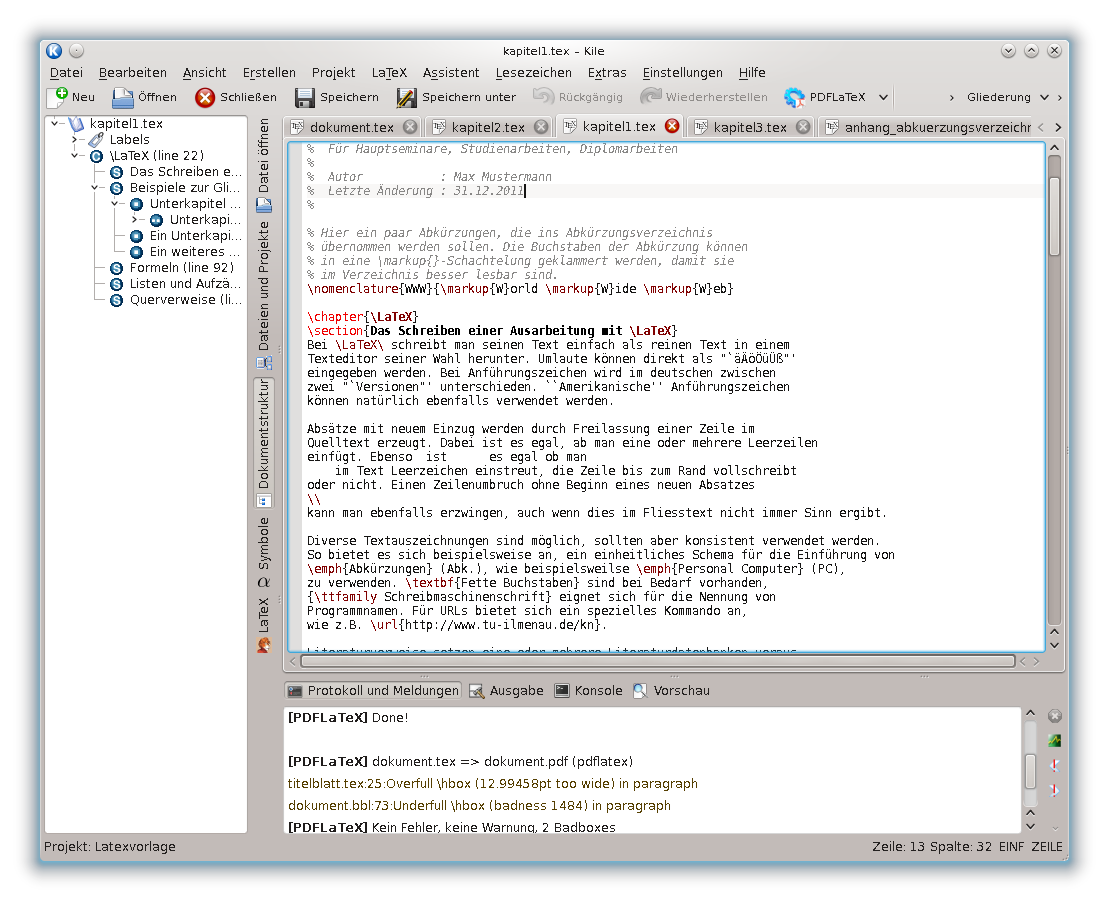
\includegraphics[width=13cm]{bilder/kile_neu.png}
\caption{Bildschirmfoto {\ttfamily kile}}
\label{bild:kile}
\end{figure}

Kile organisiert mehrere Teildokumente zu einem Projekt und
bietet damit einen einfachen Zugriff auf alle Teildokumente
einer Ausarbeitung. Syntaxhighlighting ist ebenfalls vorhanden,
sowohl für \LaTeX als auch für die BibTex"=Literaturdatenbanken.
Für den Start eines \LaTeX"=Durchlaufes sowie den verschiedenen
Konvertierungsmöglichkeiten gibt es einzelne Knöpfe. Ein direktes
Hin- und Herspringen zwischen DVI- und TEX"=Ansicht, wobei
an die korrekte Stelle gesprungen wird, ist möglich. Dies vereinfacht
Korrekturen speziell bei umfangreicheren Dokumenten.



\subsection{{\ttfamily TeXnicCenter} und {\ttfamily TeXworks} -- Windows}
Die \TeX-Entwicklungsumgebungen sind in den Bildschirmfotos \ref{bild:texniccenter} und \ref{bild:texworks} zu sehen.

\begin{figure}[!ht]
\centering
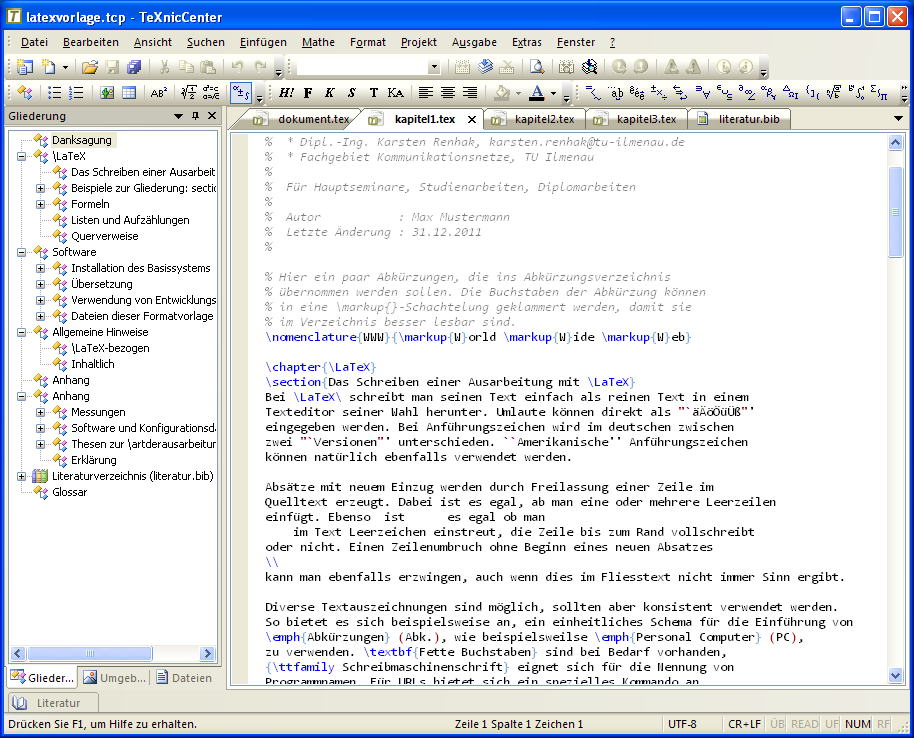
\includegraphics[width=13cm]{bilder/texniccenter_neu.png}
\caption{Bildschirmfoto {\ttfamily TeXnicCenter}}
\label{bild:texniccenter}
\end{figure}

\begin{figure}[!ht]
\centering
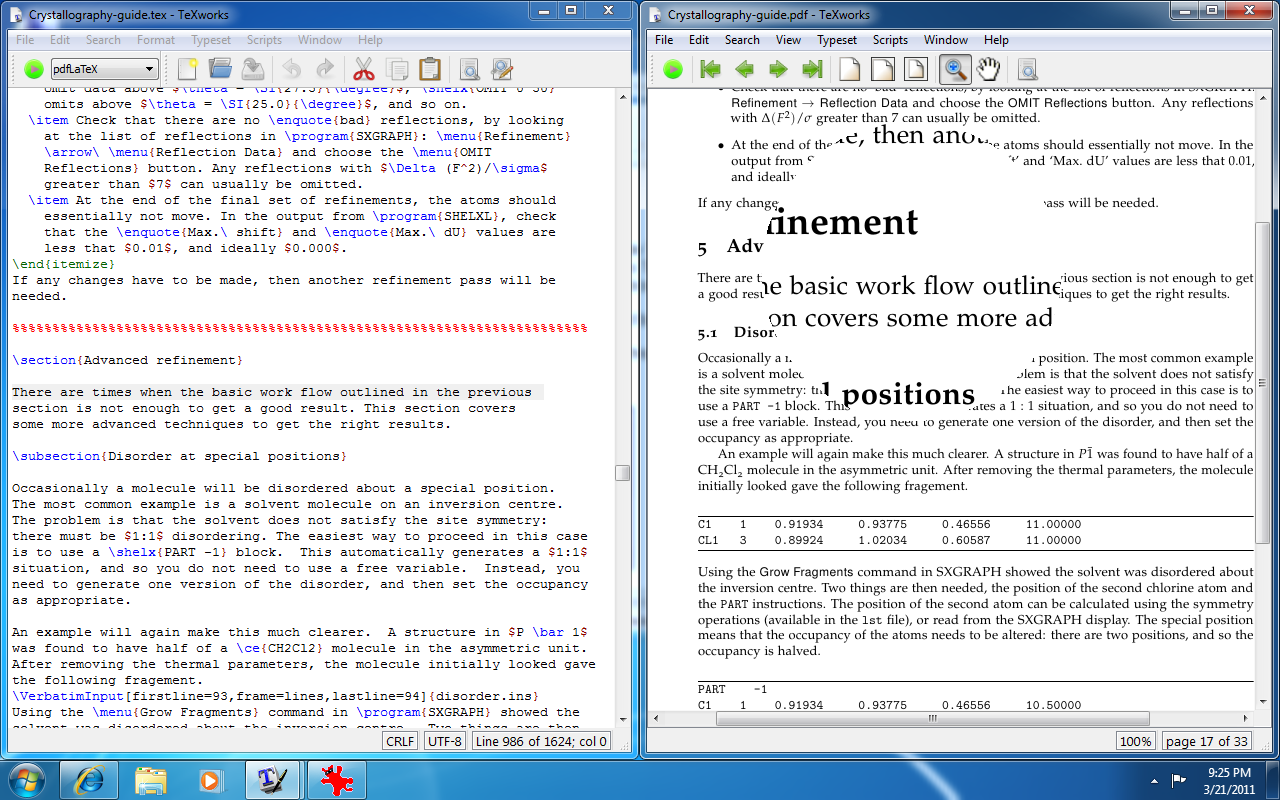
\includegraphics[width=\textwidth]{bilder/texworks-win7.png}
\caption{Bildschirmfoto {\ttfamily TeXworks}}
\label{bild:texworks}
\end{figure}



Beide Editoren bietet Syntaxhighlighting für die verschiedenen
Latexbefehle. Kurz gesagt bieten diese Entwicklungsumgebungen die
selben Features wie die im letzten Abschnitt vorgestellte
Software "`Kile."'

\textbf{Hinweis:} Wenn Sie TeXnicCenter verwenden, nutzen Sie bitte die Version 2.0 (oder größer). Zur Zeit 
(Oktober 2012) ist nur eine Alpha-Version verfügbar. Die TeXnicCenter"=Versionen 1.* unterstützen keine UTF-8 codierten Textdateien. 
Diese Vorlage ist jedoch im UTF-8 Zeichensatz \cite{wiki:utf8} gespeichert.

\nomenclature{UTF}{\markup{U}CS \markup{T}ransformation \markup{F}ormat}
\nomenclature{UCS}{\markup{U}niversal \markup{C}haracter \markup{S}et}


\section{Dateien dieser Formatvorlage}
Siehe Tabelle \ref{tabelle:dateien}.

\begin{table}[ht!]
\centering
\begin{tabular}{ll}
\hline
Dateiname &
Beschreibung
\\
\hline
{\ttfamily abschlusserklaerung.tex} &
\LaTeX\ Teildokument
\\
{\ttfamily anhang\_abbildungsverzeichnis.tex} &
\LaTeX\ Teildokument
\\
{\ttfamily anhang\_abkuerzungsverzeichnis.tex} &
\LaTeX\ Teildokument
\\
{\ttfamily anhang\_literaturverzeichnis.tex} &
\LaTeX\ Teildokument
\\
{\ttfamily anhang\_messwerte.tex} &
\LaTeX\ Teildokument
\\
{\ttfamily anhang\_programm\_a.tex} &
\LaTeX\ Teildokument
\\
{\ttfamily anhang\_programm\_b.tex} &
\LaTeX\ Teildokument
\\
{\ttfamily anhang\_protokoll.tex} &
\LaTeX\ Teildokument
\\
{\ttfamily anhang\_tabellenverzeichnis.tex} &
\LaTeX\ Teildokument
\\
{\ttfamily bilder/} &
Hier alle Bilder ablegen!
\\
{\ttfamily dokument.dvi} &
Ergebnis des \LaTeX\ Durchlaufes
\\
{\ttfamily dokument.pdf} &
Erzeugtes PDF"=Dokument
\\
{\ttfamily dokument.ps} &
Erzeugtes Postscript"=Dokument
\\
{\ttfamily dokument.tex} &
\LaTeX\ Hauptdokument
\\
{\ttfamily itmabbrv.bst} &
Formatvorlage
\\
{\ttfamily itmalpha.bst} &
Formatvorlage
\\
{\ttfamily kapitel1.tex} &
\LaTeX\ Teildokument
\\
{\ttfamily kapitel2.tex} &
\LaTeX\ Teildokument
\\
{\ttfamily kapitel3.tex} &
\LaTeX\ Teildokument
\\
{\ttfamily kurzfassung.tex} &
\LaTeX\ Teildokument
\\
{\ttfamily latexvorlage.kilepr} &
Projektdatei für {\ttfamily Kile}
\\
{\ttfamily latexvorlage.tcp} &
Projektdatei für {\ttfamily TeXnicCenter}
\\
{\ttfamily literatur.bib} &
Die Literaturdatenbank
\\
{\ttfamily thesen.tex} &
\LaTeX\ Teildokument
\\
{\ttfamily titelblatt.tex} &
\LaTeX\ Teildokument
\\
{\ttfamily vorwort.tex} &
\LaTeX\ Teildokument
\\
\hline
\end{tabular}
\caption{Relevante Dateien im Paket}
\label{tabelle:dateien}
\end{table}

